\section[Backgroud on Quantum Metrology]
{Background on Quantum Metrology}
\thiswatermark{\put(1,-241){\color{l-grey}\rule{84pt}{48pt}}
\put(84,-241){\color{grey}\rule{410pt}{48pt}}}


\quotes{Roger J. Barlow}{In the real world, doing real experiments, statistics began to matter}

\vspace{0pt}
\lettrine[lines=2, findent=3pt,nindent=0pt]{M}{etrology}, as the science of measuring, has played an essential role for the development of the technology as we know it today.
It studies several aspects of the estimation process, such as which strategy to follow in order to improve the precision of an estimation.
One of the most important figure of merit in this context is the achievable precision for a given system, independently of the strategy.
We will show how to characterize it in the subsequents sections.
And we will show as well different strategies to achieve the desired results.
The metrology science also covers from the design aspects of a precise measuring device, until the most basic concepts of nature which lead in ultimate instance to the better understanding of the whole process.

In this sense, with the discovery of the Quantum Physics and the development of Quantum Mechanics, new doors for advances in metrology were open on the earlies decades of the 19th century.
Later on, the Quantum Theory lead to the so-called field of Quantum Information which merges the notions of the theory of information and computer science, among others subfields, with the quantum mechanics.
The role of the so-named entanglement, an exclusive feature of Quantum Mechanics, is essential in this context.
Its complete understanding has integrated efforts of many researches world wide.
Said this, the entanglement also is in the center of theoretical concepts in Quantum Metrology.

On the other hand and with the aim of interpreting raw data, there are the statistics, without which many descriptions of the actual and past physical findings would lack of the rigorous interpretation needed for the complexity of data samples.



\subsection{Background on statistics and the theory of estimation}
The main mathematical tools used by the metrology science belong to statistics.
Moreover we are also interested on estimation theory.
The statistics main characteristic is that makes the raw data under consideration comprehensible from the human perspective.
The data can be anything, from a set of different heights of a basketball team, to the outcomes of a coin toss or the ages of a hundred students or even the outcomes of a thousand times repeated measurement of the electric field at some spatial point.
The aim of this section is to give the reader sufficient material to follow this thesis and make it comprehensible from the beginning.

\subsubsection{Data samples, average and variance}

As we mentioned above, everything in statistics starts with a data sample.
A data sample is defined as a set of values, we will restrict ourselves to quantitative values for simplicity, representing some magnitude.
So, in our framework such a set can be written as $X=\{x_i\}_{i=1}^M$, where all $M$ values are collected.
An illustrative example with 18 heights of different trees is shown on the Table~\ref{tab:bg-18-trees}.
\begin{table}
  \begin{center}
    \begin{tabular}{| l | c | c | c | c | c | c | c | c | c | c | c | c | c | c | c | c | c | c | }
      \hline
      Tree \# & 1 & 2 & 3 & 4 & 5 & 6 & 7 & 8 & 9 & 10 &  11 &  12 &  13 &  14 &  15 &  16 &  17 &  18
      \\ \hline
      Heights (m) & 6 &  7 &  5 &  7 &  2 & 11 &  7 &  4 &  7 &  2 &  7 &  7 &  5 &  5 &  5 &  8 &  3 & 10 \\ \hline
    \end{tabular}
  \end{center}
  \caption[Sample data of heights for trees]{A set of values for the heights of 18 trees. All measurements were rounded to integers for simplicity.}
  \label{tab:bg-18-trees}
\end{table}
It is worth to notice that this data sample represents a continuous variable, the height of some trees, while we have grouped more than a single instances into integer values.
If we would use more decimals to describe the data probably all values would have been different among each other.
This discussion is not so essential when discrete outcomes are analyzed

This picture can be extend to more outcomes coming from a single \emph{event} or measure.
For instance, a second value such as the width of the tree could be attached to each height on the previous example.
This way we have opened our approach for higher dimensional data samples that can be described as a set of $M$ outcomes with more than a single value each, $(X,Y,\dots)=\{x_i,y_i,\dots\}_{i=1}^M$.

\subsubsubsection{Average}

With this data at hand one of the first questions arises is whether the values of $X$ are around some mean value.
If one tries to address this question one of the first approaches can be computed is the \emph{arithmetic average} of the set $X$, namely,
\be
  \text{E}[X] := \frac{1}{M}\sum_{i=1}^M x_i.
\ee
Apart from the arithmetic average there are other types of averages such as the geometric mean, the root mean square or the harmonic mean, etc.
For more information see those some of those fascinating works about the statistics [XXX].
For us and for the complete understanding of this thesis will be enough with the arithmetic average.

Let us take the previous example of the trees and compute the average.
In this case the data sample is constituted by positive integer values for simplicity.
The average of the data sample is straight forward $\text{E}[X] = \frac{1}{18}\sum_{i=1}^{18} x_i = 6\text{m}$.

For the extension to the case of higher dimensional data samples one can say that each kind of outcome the average can be computed in a seamless way, $\text{E}[Y]=\frac{1}{M}\sum_{i=1}^M y_i$ and so on.

\subsubsubsection{Variance}

The second quantity one can compute is how spread the data is.
This is usually done first subtracting the average to all values on the data sample, then squaring them, so the sign of the result is lost, and finally one averages over all the resulting set. This quantity is called the \emph{variance} of the sample and it is written as follows,
\be
  \text{V}[X] := \text{E}\left[(X- \text{E}[X])^2\right],
\ee
where $X$ can be seen as a vector and when subtracting the scalar $\text{E}[X]$ and $X^2$ stands for the elements wise squared of $X$, namely $X^2 := \{x_i^2\}_{i=1}^M$.
The variance can also be written alternatively as $\text{V}[X] = \text{E}[X^2]- \text{E}[X]^2$.
The definition of the \emph{standard deviation} follows directly from the variance, $\sigma_{X}=\sqrt{\text{V}[X]}$.
Many quantities on statistics require operations like the one described right before.
This can be generalised again for more than one kind of outcome as it was done with the average.

Now let us see how result the variance for the example of the Table~\ref{tab:bg-18-trees}.
In this case the variance would be the following, $\text{V}[X]=\frac{1}{18}\sum_{i=1}^{18}x_i^2 - 6^2\text{m}^2 = 5.5\bar{5}\text{m}^2$.

To summarise and using the standard deviation, one can say now about the original distribution that most values are around 6m with a deviation of 2.357m.
Of course, some values are outside this range, but nevertheless the description is quite accurate, note that 12 values from 18 are inside the range $6\text{m}\pm2.357\text{m}$.

\subsubsubsection{Histograms}

At this point we introduce the \emph{histograms} and with that, first, the \emph{distribution function} of the data sample.
Returning to the example of the Table~\ref{tab:bg-18-trees}, one may notice that the value 7m is repeated 6 times, as the value 5m is 4 times and so on.
This is represented with the distribution function $p_i$, which in this case is for discrete values of the outcomes but which can be generalized for continuous variables as we will see later.
This function takes the value of how many times the outcome $i$ has appeared on the data sample.
Let us plot the distribution function, see Figure~\ref{fig:bg-histograms}.
\begin{figure}[tp]
  \centering
  \igwithlabel{(a)}{scale=.65}{img/plots/BG_hist_bin_1.pdf}
  \igwithlabel{(b)}{scale=.65}{img/plots/BG_hist_bin_2.pdf}
  \caption[(a) Histogram with small bin. (b) Histogram with bigger bin]{(a) $p_i$ for different values of $i$. All bars have width as 1, so it is drawn how many times each data value appears on the data sample.
  The width of the bars is called \emph{bin}, and it can change so the bars would represent a wider range of values. (b) Yo can see the same data represented in this case by a histogram with the bin size equal to 2. To produce this histogram we have summed 2 adjacent $p_i$ values starting from $p_1+p_2$, $p_3+p_4$ and so on.
  Those new bars we have chosen to represent a value in between, for instance $(3+4)/2=3.5$ and so on.}
  \label{fig:bg-histograms}
\end{figure}

Now some question arises immediately:
How this is fully connected with the previous picture?
How can one compute the average and other interesting quantities?
The answer is simple but it has to be considered carefully.
First of all, notice that $p_i$ is defined for all the natural numbers including zero, see that in the example of the trees $p_9$ equals zero, so it can be extended for other heights too setting them to zero.
This will depend on the physical property that our data sample represents but in this case it is the height of some trees, so the values cannot be negative.
Second, notice that the sum of all the repetitions, all the values of $p_i$, is exactly 18 the number of data samples in the set.
So we have that $M = \sum_{i=0}^{\infty} p_i$.
Now we can formulate the ensemble average as $\text{E}[X]=\sum_{i=0}^{\infty} p_i i / \sum_{j=0}^{\infty} p_j$. The variance and with this the standard deviation immediately follow this approach.
It is convenient to notice that the total measurement outcomes has not contribute anything but to normalize the quantities.

We can now without losing generality redefine the distribution function to be the number of repetitions corresponding to the variable divided by the total outcomes, in this case $M$.
It would have the same properties of a probability distribution function (PDF).
For instance, now we have that the sum of all $p_i$-s equal to one, $\sum_{i=0}^\infty p_i = 1$, and the average is directly obtained by computing  $\text{E}[X] = \sum_{i=0}^\infty p_i i$.
This is the approach we will follow to represent data samples.
The variance and other quantities also are simpler in this way.

\subsubsection{Probabilities and frecuentist vs. bayesian approach}

Let us talk now about probabilities.
The notion of the probability comes, [XXX].
In our contest we will define the probability in the following way.
Imagine we have an unknown data sample, let say $X$, from which we randomly choose one of the data values.
The probability to obtain a random variable $x$ is given by the parent distribution function divided by the population number $M$.

We can estimate the average height of the trees of that forest.

histogram

estimator

Explain how for bigger bin sizes, the error for higher statistical moments increases.

MLH

CLT

\subsubsection{Estimators, Fisher information}

Error propagation formula.

\subsection{Quantum Mechanics from metrology perspective}

The ubiquitous probabilistic nature of quantum mechanics forces all the community to know some basics on probability and statistics.

\subsubsubsection{The quantum state, multi-particle state, entanglement}

A \emph{system state} in Quantum Mechanics lives on a Hilbert space, $\mathcal{H}$.
The system state, $\rho$, has the following properties:
\begin{enumerate}
  \item
  It is Hermitian, so it is invariant under the complex transposition, $\rho=\rho^\dagger$.
  \item Its trace is equal to one, $\tr(\rho)=1$.
  \item It is positive semi-definite, i.e, all its eigenvalues are bigger or equal to zero, $\rho=\sum_{\lambda}p_\lambda \Pi_\lambda$\footnote{
    $\rho=\sum_{\lambda}p_\lambda \Pi_{\lambda}$ is the eigen-representation of the state, where $\Pi_{\lambda}$ are the eigenstates defined on $\mathcal{H}$ too.
    They are as many as the dimension, $d$, of the Hilbert space.
    They are orthonormal under the product defined on such Hilbert space $\mathcal{H}$, i.e, $\tr(\Pi_{\lambda}\Pi_{\lambda'})=\delta_{\lambda,\lambda'}$.
    Nevertheless, there is a extended discussion when Hilbert space is defined for continuous variables, see [XXX].
  } where $p_\lambda\geq 0$ are the scalar eigenvalues.
  It follows that $\sum_\lambda p_\lambda = 1$.
  \item If all $p_\lambda$ are zero except one, the state is a pure state, $\rho=\Pi_\lambda$.
  \item It follows that the quantum states form a convex set where the extremal points are pure states.
\end{enumerate}


The composite system of $N$ different parties lives on $\mathcal{H} = \mathcal{H}^{(1)}\otimes\mathcal{H}^{(2)}\otimes\cdots\otimes\mathcal{H}^{(N)}$ or for short $\mathcal{H} = \bigotimes_{i=1}^N\mathcal{H}^{(i)}$, where $\otimes$ stands for a tensor product like construction.
For instance, this composite Hilbert space could be used to represent a many-particle system, in this case $N$ particles.
A \emph{separable} state on this Hilbert space can be described in the following way,
\be
  \rho = \sum_{i}p_i\rho_i^{(1)}\otimes\rho_i^{(2)}\otimes\cdots\otimes\rho_i^{(N)},
\ee
where $p_i$ are convex weights that sum to one and are equal or bigger than zero.
If not the state is said to be \emph{entangled}.


Angular momentum operators.
The angular momentum algebra comes

Entanglement cannot be described classically.

Evolution

Unitary evolution

Markov

Limblad

Measurements (POVM)

Quantum Information

\subsection{Quantum Metrology}

The evolution of a quantum state can be used to infer on some hidden parameter.
The estimation theory applied to the intrinsic statistical nature of a quantum states has lead to the the formulation of Quantum Metrology as an important subfield.
Merging the probabilistic features of quantum mechanics and the estimation theory is not trivial.
Nevertheless, starting from the pioneering works of Wotters, Braunstein and some other I probably forgot to mention [XXX] were the statistical distance of neighbor states is studied we have lead to amazing results which today drive many experiments and technology.
From the works of Giovannetti et al and Paris on the middle of the last decade fundamental concepts arose, for example the figure of merit quantum Fisher information or the Heisenberg limit.
In this section we will highlight the most important aspects of this field and with this we will conclude this introductory chapter.

The error propagation formula for an estimation of $\Theta$ based on the observable $O$.
\be
  (\Delta \Theta)^2 \geq \frac{\varian{O}}{|\partial_{\Theta}\expect{O}|^2}
\ee

\subsubsection{Quantum Magnetometry}
\label{sec:bg-quantum-metro}

One of the most basic tasks of Quantum Metrology is to address the precision of estimating the magnetic field strength, namely $B$, of an unknown external magnetic field.
In this section we will assume that the magnetic field is homogeneous on the position space.
To consider more advanced situations on which the magnetic field changes linearly with the position, see chapter [XXX].
With the aim of estimating the strength of the magnetic field, a prove state is used in order to interact with it, coupling the magnetic moment of the state and the field itself.
After some time, the state has evolved.
Finally, measuring how the state has changed one would be able to infer on the strength of the magnetic field, basically proportional to the change on the state.

In general, we will say that the magnetic moments of the states come exclusively from the spin angular momentum, neglecting any possible contribution from the orbital angular momentum.
This way the physics is simpler.
This is justified in the sense that most of the recent experiments on this context have been carried out with ion-traps, BECs or at most cold atomic ensembles, which have indeed a negligible orbital angular momentum.

Beside this considerations, the interaction Hamiltonian can be written as,
\be
  H = - \bs{\mu} \cdot \bs{B}
\ee
up to some constant factor.
Now in the simplest case we will choose the magnetic field to be pointing to some fixed direction, for instance, the $z$-direction.
So the magnetic field vector can be written as ${B}=B\bs{k}$, where $\bs{k}$ is the unitary vector pointing to the $z$-direction.
This way estimation problem is much more simple, since one has not to determine the direction of the magnetic field.

The magnetic moment of the system is proportional to the spin angular momentum, $\bs{\mu}=-\mu_\text{B} g_{\text{s}}\hbar^{-1} \bs{J}$, where $\mu_{\text{B}}$ and $g_{\text{s}}$ are the Bohr magneton and anomalous gyromagnetic factor respectively.
Finally, one can rewrite the interaction Hamiltonian as,
\be
  H = \gamma B J_z
\ee
where $\gamma = \mu_\text{B} g_{\text{s}}\hbar^{-1}$ and we have used the fact that $\bs{J}\cdot\bs{k}=J_z$.
Finally, the unitary operator leading the evolution of the system can be written as,
\be
  U = \exp(-i\Theta J_z),
\ee
where the magnetic field strength is encoded into the variable $\Theta=-\mu_\text{B} g_\text{s} t B/\hbar$.
Here $\mu_\text{B}$ stand for the Magneton of Bhor and $g_\text{s}$ for the giro-magnetic constant for the spin angular momentum, and $t$ is the time spent on the evolution.

\begin{figure}
  \centering
  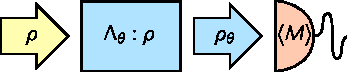
\includegraphics[scale=.85]{img/BG_preparation_encoding_estimation.pdf}
  \caption[Quantum Metrology estimation process]{Secuence of the different steps for the basics of the estimation process on Quantum Metrology. First, an input state $\rho$ enters the region on which the unknown parameter $\Theta$ is imprinted on it, for the most general case, representented with $\Lambda_{\Theta}$. Last, the state that has encoded the parameter $\Theta$ on it is measured and $\Theta$ must be infered from the measured quantity $\expect{M}$.}
  \label{fig:bg-preparation-encoding-estimation}
\end{figure}

\begin{figure}
  \centering
  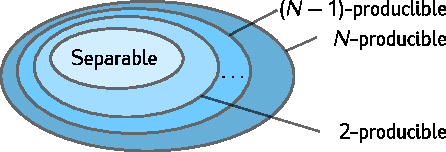
\includegraphics[scale=.85]{img/BG_separability_k_producibility_circle.pdf}
  \caption[Diagram for $k$-producibility sets]{}
  \label{fig:bg-separability-k-producibility-circle}
\end{figure}

\be
  \label{eq:bg-pezze-bound}
  \qfi[\rho,J_z] \geq \frac{\expect{J_y}^2}{\varian{J_x}}
\ee
